\chapter{Honning}
\begin{wrapfigure}{O}{0.3\linewidth}
	\centering
	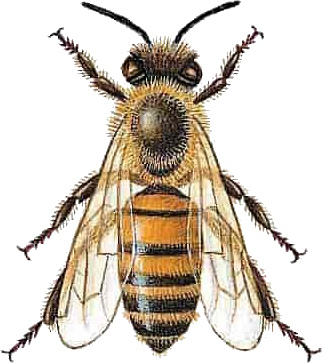
\includegraphics[width=0.8\linewidth]{honeybee.jpg}
	\caption{Illustration af \textit{Apis mellifera}-bien. Illustration af Jakob Sunesen \parencite{honneyLex}.}
	\label{fig:honeybee}
\end{wrapfigure}

Honning er et naturligt produkt lavet af \textit{A. mellifera}-bier på grundlag af plantesaft \parencite{honneyLex}.
Råmaterialerne bag honning er nektar og andet, udskilt af planter, som honningbierne indsamler, forarbejder og gemmer i deres kube.
Alle råmaterialerne kommer fra væsker i planternes sivæv, som er det væv der transporterer sukker i planten \parencite{sivævLex}.
\newline Honning kan også produceres af honningdug, som er afføring fra plantesugende insekter af ordenen næbmunde, \textit{Rhynchota} \parencite{honeybook}.
\par Efter honningbien har indsamlet råmaterialerne til fremstillingen af honning, tilføjer den i sin honningmave forskellige enzymer, mikrober og andre stoffer til honningen \parencite{sugarhoney}.
Tilbage i bikuben overfører bierne honning til vokstavlen og honningen forsegles når den er klar.
Gennem processen får honningbierne vandindholdet til at gå fra \qty{60}{\percent} til under \qty{20}{\percent} \parencite{honeybook}.
Grunden til at bierne laver nektaren om til honning, er at den ellers ville fermentere, og det er altså en måde for bierne at gemme sommerens nektar til resten af året \parencite{honeychem}.
\par Honning består primært af carbohydrater, noget vand og en lille mængde andre stoffer som phenoler, proteiner, aminosyrer, mineraler, vitaminer, pigmenter og organiske syrer \parencite{sugarhoney}.
Denne fordeling kan ses på \cref{fig:honey-comp}.
\begin{figure}[H]
	\centering
	\begin{tikzpicture}
		\pie[text=legend, change direction, rotate=90, hide number, sum=99.9, color={black!29, black!60, black!4, black!21, black!69, black!36, black!52}]{
			17.2/Vand \qty{17.2}{\percent},
			38.19/Fructose \qty{38.19}{\percent},
			31.28/Glucose \qty{31.28}{\percent},
			1.3/Sucrose \qty{1.3}{\percent},
			7.2/Maltose \qty{7.2}{\percent},
			3.24/Andet \qty{3.24}{\percent},
			1.49/Polysaccharider \qty{1.49}{\percent}
		}
		\pie[change direction, rotate=90, hide number, sum=99.9, color={black!29, black!60, black!4, black!21, black!69, black!36, black!52}]{
			17.2/\qty{17.2}{\percent},
			38.19/\qty{38.19}{\percent},
			31.28/\qty{31.28}{\percent},
			1.3/\qty{1.3}{\percent},
			7.2/\qty{7.2}{\percent},
			3.24/\qty{3.24}{\percent},
			1.49/\qty{1.49}{\percent}
		}
	\end{tikzpicture}
	\caption{Cirkeldiagram over indholdet i honning. Der vil være variation afhængig oprindelse. Fra \parencite{sugarhoney}.}
	\label{fig:honey-comp}
\end{figure}

Det skal dog noteres, at den geografiske oprindelse har meget stor betydning for honningens sammensætning \parencite{geohoney}.
Men generelt kan det siges, at honning primært består af saccharider og kun består af en meget lille bestanddel andre stoffer.
